%CHKTEX-FILE 46

\section*{Robot WALL-E Hardware Description [OPL Template]}%
\label{sec:annex-OPL}
% In this section briefly describe the software and hardware of the robot

\setlength\intextsep{0pt}
\begin{wrapfigure}[10]{r}{0.3\textwidth}
	\centering
	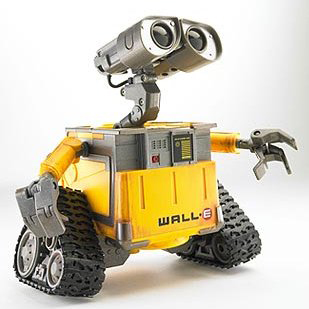
\includegraphics[width=0.4\textwidth]{images/wall-e.jpg}
	\caption{Robot WALL-E}%
	\label{fig:wall-e}
\end{wrapfigure}

Robot WALL-E has the patented \textit{Optimized Design} for garbage recollection. Specifications are as follows:

\begin{itemize}
	\item Base: all-terrain base (differential pair), 2.5m/s max speed.
	\item Torso: compressor with solar charger.
	\item Left and right arms: Mounted on torso. 7DOF, anthropomorphic. Maximum load: 20kg.
	\item Neck: telescopic neck with pan and tilt.
	\item Head: 3DOF Expressive Eyes
	\item Robot dimensions: height: 1.2m (max), width: 0.7m depth 0.8m
	\item Robot weight: 50kg.
\end{itemize}

\noindent\textit{Also our robot incorporates the following devices:}

\begin{itemize}
	\item Battery charge indicator
	\item Auto-focus all-purpose cameras
	\item 7DOF heavy duty fingers
	\item Cockroach
\end{itemize}

\section*{Robot's Software Description}
% Please describe in this section the software you are using to control your robot. Consider the following example:

\textit{For our robot we are using the following software:}

\begin{itemize}
	\item Platform: Operating System
	\item Navigation: Navigator
	\item Face recognition: None. Not designed for human interaction.
	\item Speech recognition: All-purpose recognizer~\cite{bnl1}.
	\item Speech generation: None. Not designed for human interaction.
	\item Object recognition: Trash Seeker Algorithm (See previous sections).
	\item Arms control and two-hand coordination: automatic controller~\cite{bnl2}.
\end{itemize}

\section*{External Devices}
% Please describe in this section the external devices used by your robot. Consider the following example:

\textit{WALL-E robot relies on the following external hardware:}

\begin{itemize}
	\item Garbage Compactor
	\item EVA unit
	\item Data Cluster
	\item $3 \times$ Ultra-Power laptops.
\end{itemize}

\section*{Cloud Services}
% Please describe in this section the Cloud Services and online software used by your robot. Consider the following example:

\textit{WALL-E connects the following cloud services:}
\begin{itemize}
	\item Localization and mapping: Geolocalization system~\cite{bnl3}.
\end{itemize}